%In this section we outline our methodology for designing a system that can predict the execution
%time SLAs of web APIs developed for cloud platforms.
We start by making several observations regarding PaaS clouds. First and foremost, 
they require developers
to implement applications using a predefined set of programming interfaces. When considered as a
collection, we shall refer to these programming interfaces as the cloud software development 
kit or the \textit{cloud SDK}. We refer to the individual member interfaces of the cloud SDK
as \textit{cloud SDK interfaces}, and their constituent operations are referred to as \textit{cloud SDK operations}.

%Lets further elaborate this notion by taking Google App Engine~\cite{gae}, one of the earliest and most widely
%used PaaS clouds, as a concrete example. 
Google App Engine, for example, provides several cloud SDKs; one for each
programming language supported (Java, Python, Go etc). Each SDK consists of
several cloud SDK interfaces. Table~\ref{tab:gae_cloud_sdk} lists some of them.
Each individual interface is comprised of several cloud SDK operations. For instance, the 
datastore interface of App Engine provides operations for saving an entity (a data object),
deleting an entity and querying the datastore to read one or more entities.

\begin{table}[htdp]
\caption{Google App Engine cloud SDK interfaces}
\begin{center}
\begin{tabular}{|c|p{5cm}|}
\hline
Cloud SDK Interface & Functionality \\ \hline
datastore & Reading and writing data to a highly scalable database with some transaction support. \\ \hline
memcache & In-memory caching of data for faster access.\\ \hline
users & User session management (login and logout)\\ \hline
blobstore & Reading and writing large chunks (blobs) of uninterpreted bytes.\\ \hline
task queue & Scheduling periodic and background jobs.\\ \hline
\end{tabular}
\end{center}
\label{tab:gae_cloud_sdk}
\end{table}

\begin{figure}
\centering
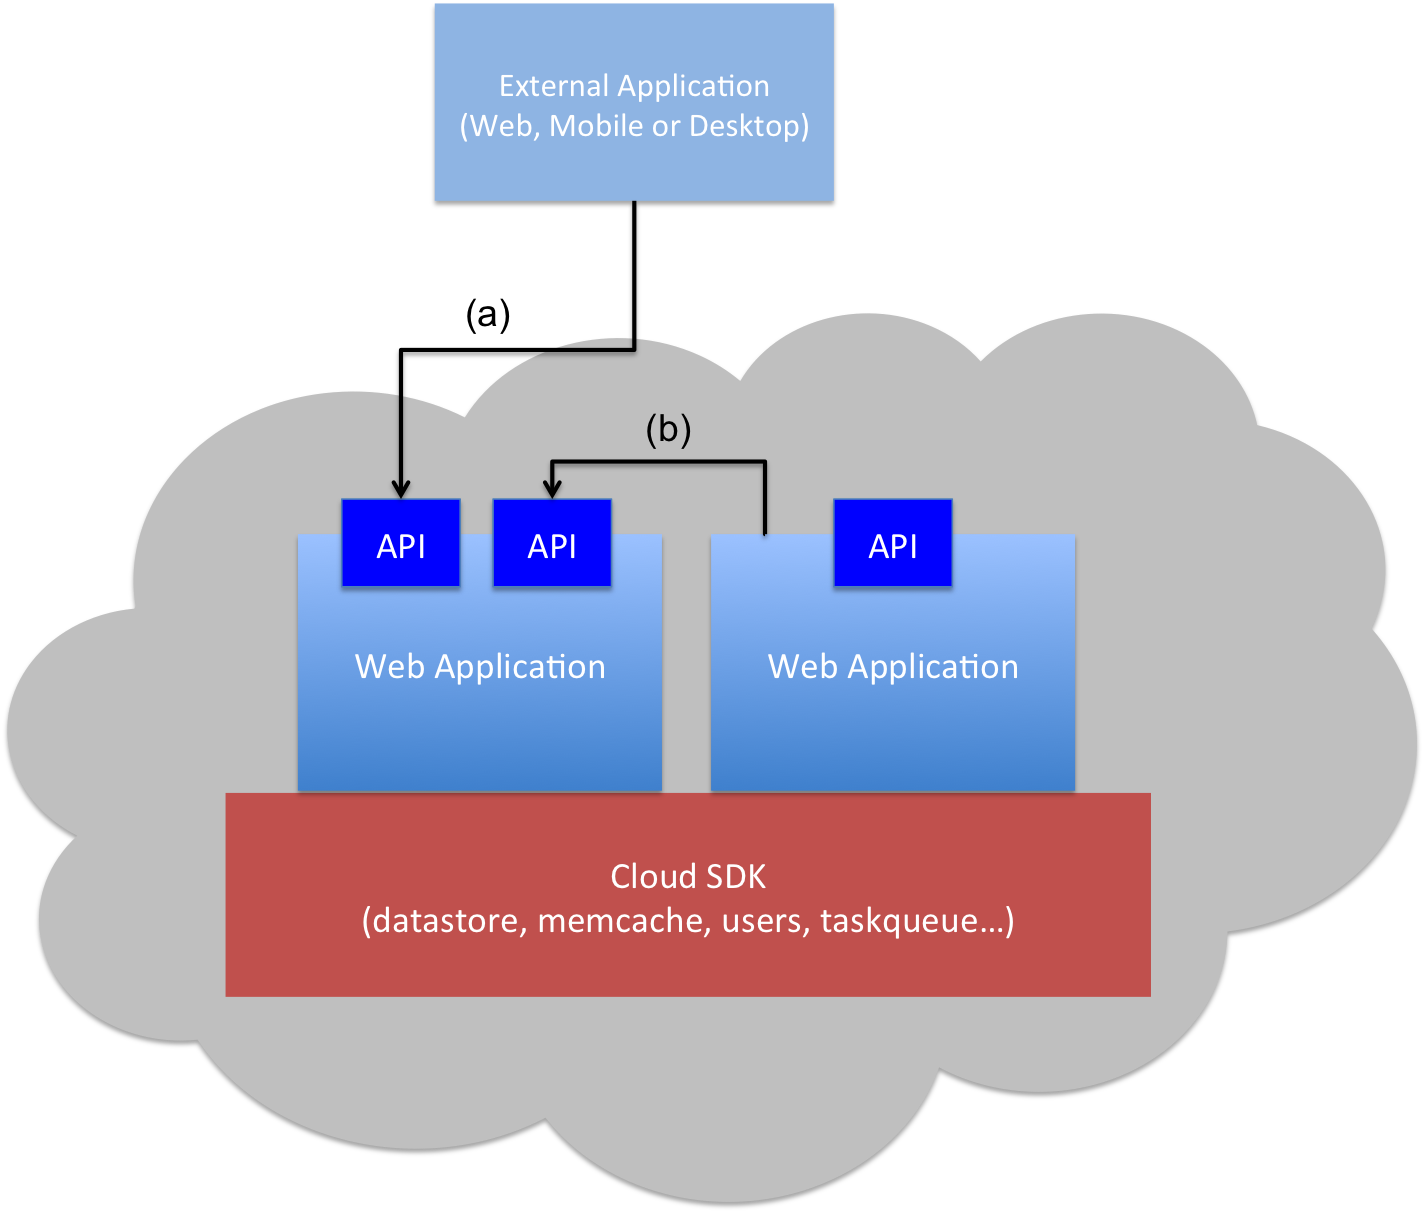
\includegraphics[scale=0.35]{cloud_app_model}
\caption{Applications and APIs deployed in a PaaS cloud: (a) An external application invoking a web API hosted in the cloud. 
(b) An application hosted in the PaaS cloud invoking a web API hosted in the same cloud.}
\label{fig:cloud_app_model}
\end{figure}

Figure~\ref{fig:cloud_app_model} illustrates the application and API deployment model supported in PaaS clouds.
Developers implement web applications using the cloud SDK. These web applications may contain zero or more
web APIs. Web APIs themselves are comprised of executable code. 
Developers then use these web APIs (over the network) to create new applications that are executed elsewhere or within the
same cloud.

Cloud SDKs facilitate a wide range of useful application features like data management, 
task scheduling and security. Therefore we can expect any web API developed for the cloud to
contain some number of cloud SDK calls -- i.e.
explicit invocations of cloud SDK operations. Since these invocations need to be handled by the
underlying cloud platform, their overhead is higher than the locally executed operations.
Hence, we can expect cloud web API codes to spend most of their execution time on cloud SDK operations. 

The above prospect is further supported by the fact that PaaS clouds do not allow 
certain types of operations in the application code. Such restrictions are in place
to ensure scalability, stability and security of the cloud platform. For example, App Engine
does not provide access to the local file system. %Since PaaS applications run on a shared cloud
%platform and not on dedicated machines, there is no clear notion of a local file system in such environments.
%Also file system operations are slow and do not scale.
Hence, the developers must use the datastore and blobstore cloud SDK interfaces on App
Engine to implement functionality equivalent to file I/O. Similarly, App Engine provides cloud SDK
interfaces like urlfetch, sockets, xmpp and mail that can replace a lot of network I/O code.

The mandated use of cloud SDK operations in the applications, and their relatively high overhead 
imply that we can use the cloud SDK
invocations made by the web API implementations as an indicator of their performance. Intuitively, a web API
code that makes a large number of cloud SDK invocations can be expected to run slowly compared
to an API that only makes a few cloud SDK invocations. Based on this idea, we propose the following approach
for designing a system that can estimate the execution time of cloud web APIs:

\begin{itemize}
\item We run a monitoring agent in the cloud platform to track the performance of
cloud SDK operations over time. This agent should always execute in the cloud, collecting
cloud SDK performance data in the background. %Note that it does not monitor any of the
%deployed applications. Rather, it independently benchmarks the cloud SDK operations.
\item Given a web API code, we statically analyze it to identify the set of cloud SDK operations
invoked by the code. We assume that the type and the number of cloud SDK calls made by the API implementation
are the only factors that determine how fast the web API can execute. We ignore all other local operations
as not contributing to the API execution time.
\item We combine the cloud SDK invocations extracted from the web API code with the historical
performance data collected on those cloud SDK operations to estimate an upper bound for the
execution time of web API code. By making the estimation somewhat conservative, we can offset 
any differences in the actual execution time caused by the parts of the code that are ignored during
static analysis. 
\end{itemize}

The proposed approach allows us to estimate the execution time of web APIs without having to
run the API code.
In fact, we can carry out the static analysis and the subsequent execution time
estimation before we even deploy the application to the cloud. 
This means we can \textit{predict} the SLAs that can be supported by a given web API code
without running any load tests on it. 
%Such a system would be very useful and
%easy to use for both API developers and cloud administrators. It enables API developers
%to advertise precise SLAs regarding the performance of their APIs, from day one. It enables
%cloud administrators to enforce performance-related policies and make sure that all deployed 
%web APIs adhere to certain standards when it comes to their execution times.

Web APIs developed for PaaS clouds have several qualities that make our proposal
feasible and even attractive.

\begin{itemize}
\item PaaS clouds do not support codes that take too long to execute or do not terminate. For 
example, in App Engine all codes must finish executing under 60 seconds.
%The platform forcefully terminates any thread that runs longer than the allowed time period.
Therefore our static analysis does not need to bother about the termination of any given web API
code. The hard deadline also means we have a worst-case SLA for all web APIs to begin with.
\item Web API implementations are essentially HTTP request processing codes. We can expect them
to fit the general model of $receive\_request \Rightarrow process \Rightarrow send\_response$. In
other words, the codes we need to analyze have definite starting and finishing points that are easier
to identify.
\item PaaS clouds enforce a restricted thread model on the application code. Again, if we take
App Engine as an example, it does not allow creating new threads in the application code. This
makes it possible to statically reason about the concurrent execution behavior of the code.
%\item PaaS clouds do not support developing codes with arbitrary third party libraries. Instead they
%publish a whitelist of supported libraries. This also makes it easier to statically analyze the form of web API codes.
\end{itemize}

To further understand the characteristics of cloud applications, and how we can leverage them,
we conduct a survey
using a collection of real world PaaS applications. In the next section we present the major findings
of this survey.
%In the sections that follow we describe how we designed and implemented Cerebro, a system based on
%the proposed approach for predicting web API performance SLAs.